\documentclass[11pt]{book}
%\oddsidemargin 0in
%\evensidemargin 0in
%\marginparwidth 0in

%\usepackage[top=1in
%,left=1.5in,
%bottom=1in,%right=1in,textheight=8.5in,textwidth=6in
%]{geometry}

\usepackage{amsfonts,amssymb,amsmath,amsthm,fancyhdr,supertabular,longtable,hhline}
\usepackage{colortbl}
\usepackage{docmute}
\usepackage{import, multicol,boxedminipage}
\usepackage{chapterfolder}
\usepackage[metapost,truebbox]{mfpic}
\usepackage[pdflatex]{graphicx}
\usepackage{graphics}
\usepackage{pgf, tikz}
\usepackage[matrix,arrow,curve]{xy}
\usepackage{setspace}
\usepackage{makeidx}
\usepackage{nomencl}
\usepackage[english]{babel}
\usepackage[colorlinks, hyperindex, plainpages=false, linkcolor=blue, urlcolor=blue, pdfpagelabels]{hyperref}
\usepackage[all]{hypcap}
\usepackage{cancel}
\usepackage{sectsty}
\usepackage{textcomp}
\usepackage{array}
\usepackage{vwcol}
\usepackage{cancel}
\usepackage[
type={CC},
modifier={by-nc-sa},
version={4.0},
]{doclicense}
%\usepackage{bbm}

%First appears in II.1.1
\newcommand{\tmdummy}{$\mbox{}$}
\newcommand{\tmmathbf}[1]{\ensuremath{\boldsymbol{#1}}}
\newcommand{\tmop}[1]{\ensuremath{\operatorname{#1}}}
\newcommand{\tmstrong}[1]{\textbf{#1}}
%{\theorembodyfont{\rmfamily}
%First appears in II.1.?
\newcommand{\tmem}[1]{{\em #1\/}}
%\newenvironment{enumeratenumeric}{\begin{enumerate}[1.] }{\end{enumerate}}
%First appears in II.1.6a
\newenvironment{itemizedot}{\begin{itemize} \renewcommand{\labelitemi}{$\bullet$}\renewcommand{\labelitemii}{$\bullet$}\renewcommand{\labelitemiii}{$\bullet$}\renewcommand{\labelitemiv}{$\bullet$}}{\end{itemize}}


\allsectionsfont{\mdseries \scshape}
\definecolor{ResultColor}{gray}{1.0} %SZ set to gray, 0.9
\theoremstyle{definition}  % this prevents the text in definitions, theorems, and corollaries from being italicized
\newtheorem*{defn}{Definition}%[chapter] % this item asterisked for numbering purposes (across all chapters).
%\newtheorem*{thm}{Theorem}%[chapter] % this item asterisked for numbering purposes (across all chapters).
\newtheorem{thm}{Theorem}[chapter] % this item asterisked for numbering purposes (across all chapters).
\newtheorem*{cor}%[thm]
{Corollary} % this item asterisked for numbering purposes (across all chapters).
\newtheorem{eqn}{Equation}[chapter]
\newtheorem{ex}{Example}[chapter] % this is needed for all Stitz Zeager content.
\newtheorem{example}{Example}[chapter]
\newtheorem{fig}{\sc Figure}[chapter]
\setlength{\parindent}{0in}
\setlength{\extrarowheight}{2pt}
\newcommand{\bbm}{\begin{boxedminipage}{4.80in}} %SZ set to 6.41
\newcommand{\ebm}{\end{boxedminipage}}
\newcounter{HW}
\newcounter{HWindent}

\newcommand{\comment}[1]{}
\newcommand{\pp}{\par~\par}

\begin{document}

\subsection{Solving Linear Equations}\par

\subsubsection{One-Step Equations}\par

%\maketitle \ \ \ \ \ \ \ \ \ \ \ \ \ \ \ \ \ \ \ \ \ \ \ \ \ \ \ \ \ \ \ \ \ \
%\ \ \ \ \ \ \ \ \ \ \ \ \ \ \ \ \ \ \ \

{\tmstrong{Solve each equation.}}

\begin{multicols}{2}
  1) $v + 9 = 16$ \ \ \ \ \ \ \ \ \ \ \ \ \ \ \ \ \ \ \
  
  3)$x - 11 = - 16$ \ \ \ \ \ \ \ \ \ \ \ \ \ \ \ \ \ \ \ \ \ \ \ \ \ \ \ \
  
  5) $30 = a + 20$ \ \ \ \ \ \ \ \ \ \ \ \ \ \ \ \ \ \ \ \ \ \ \ \ \ \ \ \ \
  \ \
  
  7) $x - 7 = - 26$ \ \ \ \ \ \ \ \ \ \ \ \ \ \ \ \ \ \ \ \ \ \ \ \ \ \ \ \ \
  \
  
  9) $13 = n - 5$ \ \ \ \ \ \ \ \ \ \ \ \ \ \ \ \ \ \ \ \ \ \ \ \ \ \ \ \ \ \
  \ \ \
  
  11) $340 = - 17 x$ \ \ \ \ \ \ \ \ \ \ \ \ \ \ \ \ \ \ \ \ \ \ \ \ \ \ \ \
  \
  
  13) $- 9 = \frac{n}{12}$ \ \ \ \ \ \ \ \ \ \ \ \ \ \ \ \ \ \ \ \ \ \ \ \ \
  \ \ \ \ \ \ \ \ \
  
  15) $20 v = - 160$ \ \ \ \ \ \ \ \ \ \ \ \ \ \ \ \ \ \ \ \ \ \ \ \ \ \ \ \
  \
  
  17) $340 = 20 n$ \ \ \ \ \ \ \ \ \ \ \ \ \ \ \ \ \ \ \ \ \ \ \ \ \ \ \ \ \
  \ \ \
  
  19) $16 x = 320$ \ \ \ \ \ \ \ \ \ \ \ \ \ \ \ \ \ \ \ \ \ \ \ \ \ \ \ \ \
  \
  
  21) $- 16 + n = - 13$ \ \ \ \ \ \ \ \ \ \ \ \ \ \ \ \ \ \ \ \ \ \ \
  
  23) $p - 8 = - 21$ \ \ \ \ \ \ \ \ \ \ \ \ \ \ \ \ \ \ \ \ \ \ \ \ \ \ \
  
  25) $180 = 12 x$ \ \ \ \ \ \ \ \ \ \ \ \ \ \ \ \ \ \ \ \ \ \ \ \ \ \ \ \ \
  \ \
  
  27) $20 b = - 200$ \ \ \ \ \ \ \ \ \ \ \ \ \ \ \ \ \ \ \ \ \ \ \ \ \ \ \ \
  \
  
  29) $\frac{r}{14} = \frac{5}{14}$ \ \ \ \ \ \ \ \ \ \ \ \ \ \ \ \ \ \ \ \ \
  \ \ \ \ \ \ \ \ \ \ \ \ \
  
  31) $- 7 = a + 4$ \ \ \ \ \ \ \ \ \ \ \ \ \ \ \ \ \ \ \ \ \ \ \ \ \ \ \ \ \
  
  33) $10 = x - 4$ \ \ \ \ \ \ \ \ \ \ \ \ \ \ \ \ \ \ \ \ \ \ \ \ \ \ \ \ \
  \ \
  
  35) $13 a = - 143$ \ \ \ \ \ \ \ \ \ \ \ \ \ \ \ \ \ \ \ \ \ \ \ \ \ \ \ \
  \
  
  37) $\frac{p}{20} = - 12$ \ \ \ \ \ \ \ \ \ \ \ \ \ \ \ \ \ \ \ \ \ \ \ \ \
  \ \ \ \ \ \ \ \
  
  39) $9 + m = - 7$ \ \ \ \ \ \ \ \ \ \ \ \ \ \ \ \ \ \ \ \ \ \ \ \ \ \ \ \ \
  \ \ \ \ \ \ \ \
  
  2) $14 = b + 3$
  
  4) $- 14 = x - 18$
  
  6) $- 1 + k = 5$
  
  8) $- 13 + p = - 19$
  
  10) $22 = 16 + m$
  
  12) $4 r = - 28$
  
  14) $\frac{5}{9} = \frac{b}{9}$
  
  16) $- 20 x = - 80$
  
  18) $\frac{1}{2} = \frac{a}{8}$
  
  20) $\frac{k}{13} = - 16$
  
  22) $21 = x + 5$
  
  24) $m - 4 = - 13$
  
  26) $3 n = 24$
  
  28) $- 17 = \frac{x}{12}$
  
  30) $n + 8 = 10$
  
  32) $v - 16 = - 30$
  
  34) $- 15 = x - 16$
  
  36) $- 8 k = 120$
  
  38) $- 15 = \frac{x}{9}$
  
  40) $- 19 = \frac{n}{20}$
\end{multicols}

\vspace{2in}
~

\pagebreak

\subsubsection{Two-Step Equations}\par

%\maketitle \ \ \ \ \ \ \ \ \ \ \ \ \ \ \ \ \ \ \ \ \ \ \ \ \ \ \ \ \ \ \ \ \ \
%\ \ \ \ \ \ \ \ \ \ \ \ \ \ \

{\tmstrong{Solve each equation.}}

\begin{multicols}{2}
  1) $5 + \frac{n}{4} = 4$ \ \ \ \ \ \ \ \ \ \ \ \ \ \ \ \ \ \ \ \ \ \ \ \ \ \
  \ \ \ \ \ \ \
  
  3) $102 = - 7 r + 4$ \ \ \ \ \ \ \ \ \ \ \ \ \ \ \ \ \ \ \ \ \ \ \ \ \ \ \
  
  5) $- 8 n + 3 = - 77$ \ \ \ \ \ \ \ \ \ \ \ \ \ \ \ \ \ \ \ \ \ \ \ \ \
  
  7) $0 = - 6 v$ \ \ \ \ \ \ \ \ \ \ \ \ \ \ \ \ \ \ \ \ \ \ \ \ \ \ \ \ \ \
  \ \ \ \
  
  9) $- 8 = \frac{x}{5} - 6$ \ \ \ \ \ \ \ \ \ \ \ \ \ \ \ \ \ \ \ \ \ \ \ \
  \ \ \ \ \ \
  
  11) $0 = - 7 + \frac{k}{2}$ \ \ \ \ \ \ \ \ \ \ \ \ \ \ \ \ \ \ \ \ \ \ \ \
  \ \ \ \ \
  
  13) $- 12 + 3 x = 0$ \ \ \ \ \ \ \ \ \ \ \ \ \ \ \ \ \ \ \ \ \ \ \ \ \ \
  
  15) $24 = 2 n - 8$ \ \ \ \ \ \ \ \ \ \ \ \ \ \ \ \ \ \ \ \ \ \ \ \ \ \ \ \
  \
  
  17) $2 = - 12 + 2 r$ \ \ \ \ \ \ \ \ \ \ \ \ \ \ \ \ \ \ \ \ \ \ \ \ \ \ \
  
  19) $\frac{b}{3} + 7 = 10$ \ \ \ \ \ \ \ \ \ \ \ \ \ \ \ \ \ \ \ \ \ \ \ \
  \ \ \ \ \ \ \
  
  21) $152 = 8 n + 64$ \ \ \ \ \ \ \ \ \ \ \ \ \ \ \ \ \ \ \ \ \ \ \ \ \ \ \
  
  23) $- 16 = 8 a + 64$ \ \ \ \ \ \ \ \ \ \ \ \ \ \ \ \ \ \ \ \ \ \ \ \ \
  
  25) $56 + 8 k = 64$ \ \ \ \ \ \ \ \ \ \ \ \ \ \ \ \ \ \ \ \ \ \ \ \ \ \ \ \
  \
  
  27) $- 2 x + 4 = 22$ \ \ \ \ \ \ \ \ \ \ \ \ \ \ \ \ \ \ \ \ \ \ \ \ \ \ \
  
  29) $- 20 = 4 p + 4$ \ \ \ \ \ \ \ \ \ \ \ \ \ \ \ \ \ \ \ \ \ \ \ \ \ \ \
  
  31) $- 5 = 3 + \frac{n}{2}$ \ \ \ \ \ \ \ \ \ \ \ \ \ \ \ \ \ \ \ \ \ \ \ \
  \ \ \ \ \
  
  33) $\frac{r}{8} - 6 = - 5$ \ \ \ \ \ \ \ \ \ \ \ \ \ \ \ \ \ \ \ \ \ \ \ \
  \ \ \ \ \
  
  35) $- 40 = 4 n - 32$ \ \ \ \ \ \ \ \ \ \ \ \ \ \ \ \ \ \ \ \ \ \ \ \
  
  37) $87 = 3 - 7 v$ \ \ \ \ \ \ \ \ \ \ \ \ \ \ \ \ \ \ \ \ \ \ \ \ \ \ \ \
  \ \
  
  39) $- x + 1 = - 11$ \ \ \ \ \ \ \ \ \ \ \ \ \ \ \ \ \ \ \ \ \ \ \ \ \ \ \
  \ \ \ \ \ \ \ \ \
  
  2) $- 2 = - 2 m + 12$
  
  4) $27 = 21 - 3 x$
  
  6) $- 4 - b = 8$
  
  8) $- 2 + \frac{x}{2} = 4$
  
  10) $- 5 = \frac{a}{4} - 1$
  
  12) $- 6 = 15 + 3 p$
  
  14) $- 5 m + 2 = 27$
  
  16) $- 37 = 8 + 3 x$
  
  18) $- 8 + \frac{n}{12} = - 7$
  
  20) $\frac{x}{1} - 8 = - 8$
  
  22) $- 11 = - 8 + \frac{v}{2}$
  
  24) $- 2 x - 3 = - 29$
  
  26) $- 4 - 3 n = - 16$
  
  28) $67 = 5 m - 8$
  
  30) $9 = 8 + \frac{x}{6}$
  
  32) $\frac{m}{4} - 1 = - 2$
  
  34) $- 80 = 4 x - 28$
  
  36) $33 = 3 b + 3$
  
  38) $3 x - 3 = - 3$
  
  40) $4 + \frac{a}{3} = 1$
\end{multicols}

\vspace{2in}
~

\pagebreak

\subsubsection{General Linear Equations}\par

{\tmstrong{Solve each equation.}}

\begin{multicols}{2}
  1) $2 - (- 3 a - 8) = 1$ \ \ \ \ \ \ \ \ \ \
  
  3) $- 5 (- 4 + 2 v) = - 50$ \ \ \ \ \ \ \ \ \ \
  
  5) $66 = 6 (6 + 5 x) $ \ \ \ \ \ \ \ \ \ \ \ \ \ \ \ \ \ \ \ \
  
  7) $0 = - 8 (p - 5)$ \ \ \ \ \ \ \ \ \ \ \ \ \ \ \ \ \ \ \ \ \ \ \
  
  9) $- 2 + 2 (8 x - 7) = - 16$ \ \ \ \ \ \ \ \ \ \ \
  
  11) $- 21 x + 12 = - 6 - 3 x$ \ \ \ \ \ \ \ \ \ \ \ \ \ \
  
  13) $- 1 - 7 m = - 8 m + 7$ \ \ \ \ \ \ \ \ \ \ \ \ \ \
  
  15) $1 - 12 r = 29 - 8 r$ \ \ \ \ \ \ \ \ \ \ \ \ \ \ \
  
  17) $20 - 7 b = - 12 b + 30$ \ \ \ \ \ \ \ \ \ \ \ \ \ \ \ \ \
  
  19) $- 32 - 24 v = 34 - 2 v$ \ \ \ \ \ \ \ \ \ \ \ \
  
  21) $- 2 - 5 (2 - 4 m) = 33 + 5 m$ \ \ \ \ \ \ \ \
  
  23) $- 4 n + 11 = 2 (1 - 8 n) + 3 n$ \ \ \ \ \ \
  
  25) $- 6 v - 29 = - 4 v - 5 (v + 1) $ \ \ \ \ \ \
  
  27) $2 (4 x - 4) = - 20 - 4 x$ \ \ \ \ \ \ \ \ \ \ \ \ \
  
  29) $- a - 5 (8 a - 1) = 39 - 7 a$ \ \ \ \ \ \ \
  
  31) $- 57 = - (- p + 1) + 2 (6 + 8 p)$ \ \ \ \
  
  33) $- 2 (m - 2) + 7 (m - 8) = - 67$ \ \ \
  
  35) $50 = 8 (7 + 7 r) - (4 r + 6)$ \ \ \ \ \ \ \ \
  
  37) $- 8 (n - 7) + 3 (3 n - 3) = 41$ \ \ \ \ \ \ \
  
  39) $- 61 = - 5 (5 r - 4) + 4 (3 r - 4)$ \
  
  41) $- 2 (8 n - 4) = 8 (1 - n)$ \ \ \ \ \ \ \ \ \ \ \ \
  
  43) $- 3 (- 7 v + 3) + 8 v = 5 v - 4 (1 - 6 v) $
  
  45) $- 7 (x - 2) = - 4 - 6 (x - 1)$ \ \ \ \ \ \ \ \ \
  
  47) $- 6 (8 k + 4) = - 8 (6 k + 3) - 2$ \ \ \ \ \
  
  49) $- 2 (1 - 7 p) = 8 (p - 7)$ \ \ \ \ \ \ \ \ \ \ \ \
  
  2) $2 (- 3 n + 8) = - 20$
  
  4) $2 - 8 (- 4 + 3 x) = 34$
  
  6) $32 = 2 - 5 (- 4 n + 6)$
  
  8) $- 55 = 8 + 7 (k - 5)$
  
  10) $- (3 - 5 n) = 12$
  
  12) $- 3 n - 27 = - 27 - 3 n$
  
  14) $56 p - 48 = 6 p + 2$
  
  16) $4 + 3 x = - 12 x + 4$
  
  18) $- 16 n + 12 = 39 - 7 n$
  
  20) $17 - 2 x = 35 - 8 x$
  
  22) $- 25 - 7 x = 6 (2 x - 1)$
  
  24) $- 7 (1 + b) = - 5 - 5 b$
  
  26) $- 8 (8 r - 2) = 3 r + 16$
  
  28) $- 8 n - 19 = - 2 (8 n - 3) + 3 n$
  
  30) $- 4 + 4 k = 4 (8 k - 8)$
  
  32) $16 = - 5 (1 - 6 x) + 3 (6 x + 7)$
  
  34) $7 = 4 (n - 7) + 5 (7 n + 7)$
  
  36) $- 8 (6 + 6 x) + 4 (- 3 + 6 x) = - 12$
  
  38) $- 76 = 5 (1 + 3 b) + 3 (3 b - 3)$
  
  40) $- 6 (x - 8) - 4 (x - 2) = - 4$
  
  42) $- 4 (1 + a) = 2 a - 8 (5 + 3 a) $
  
  44) $- 6 (x - 3) + 5 = - 2 - 5 (x - 5)$
  
  46) $- (n + 8) + n = - 8 n + 2 (4 n - 4)$
  
  48) $- 5 (x + 7) = 4 (- 8 x - 2)$
  
  50) $8 (- 8 n + 4) = 4 (- 7 n + 8)$
\end{multicols}

\vspace{1.5in}
~

\pagebreak

\subsubsection{Equations Containing Fractions}\par

{\tmstrong{Solve each equation.}}

\begin{multicols}{2}
  1) $\frac{3}{5} (1 + p) = \frac{21}{20}$
  
  3) $0 = - \frac{5}{4} (x - \frac{6}{5})$
  
  5) $\frac{3}{4} - \frac{5}{4} m = \frac{113}{24}$
  
  7) $\frac{635}{72} = - \frac{5}{2} (- \frac{11}{4} + x)$
  
  9) $2 b + \frac{9}{5} = - \frac{11}{5}$
  
  11) $\frac{3}{2} (\frac{7}{3} n + 1) = \frac{3}{2}$
  
  13) $- a - \frac{5}{4} (- \frac{8}{3} a + 1) = - \frac{19}{4}$
  
  15) $\frac{55}{6} = - \frac{5}{2} (\frac{3}{2} p - \frac{5}{3})$
  
  17) $\frac{16}{9} = - \frac{4}{3} (- \frac{4}{3} n - \frac{4}{3})$
  
  19) $- \frac{5}{8} = \frac{5}{4} (r - \frac{3}{2})$
  
  21) $- \frac{11}{3} + \frac{3}{2} b = \frac{5}{2} (b - \frac{5}{3})$
  
  23) $- (- \frac{5}{2} x - \frac{3}{2}) = - \frac{3}{2} + x$
  
  25) $\frac{45}{16} + \frac{3}{2} n = \frac{7}{4} n - \frac{19}{16}$
  
  27) $\frac{3}{2} (v + \frac{3}{2}) = - \frac{7}{4} v - \frac{19}{6}$
  
  29) $\frac{47}{9} + \frac{3}{2} x = \frac{5}{3} (\frac{5}{2} x_{} + 1)$\\
  
  2) $- \frac{1}{2} = \frac{3}{2} k + \frac{3}{2}$
  
  4) $\frac{3}{2} n - \frac{8}{3} = - \frac{29}{12}$
  
  6) $\frac{11}{4} + \frac{3}{4} r = \frac{163}{32}$
  
  8) $- \frac{16}{9} = - \frac{4}{3} (\frac{5}{3} + n)$
  
  10) $\frac{3}{2} - \frac{7}{4} v = - \frac{9}{8}$
  
  12) $\frac{41}{9} = \frac{5}{2} (x + \frac{2}{3}) - \frac{1}{3} x$
  
  14) $\frac{1}{3} (- \frac{7}{4} k + 1) - \frac{10}{3} k = - \frac{13}{8}$
  
  16)$- \frac{1}{2} (\frac{2}{3} x - \frac{3}{4}) - \frac{7}{2} x = -
  \frac{83}{24}$
  
  18) $\frac{2}{3} (m + \frac{9}{4}) - \frac{10}{3} = - \frac{53}{18}$
  
  20) $\frac{1}{12} = \frac{4}{3} x + \frac{5}{3} (x - \frac{7}{4})$
  
  22) $\frac{7}{6} - \frac{4}{3} n = - \frac{3}{2} n + 2 (n + \frac{3}{2})$
  
  24) $- \frac{149}{16} - \frac{11}{3} r \text{=} - \frac{7}{4} r -
  \frac{5}{4} (- \frac{4}{3} r + 1)$
  
  26) $- \frac{7}{2} (\frac{5}{3} a + \frac{1}{3}) = \frac{11}{4} a +
  \frac{25}{8}$
  
  28) $- \frac{8}{3} - \frac{1}{2} x = - \frac{4}{3} x - \frac{2}{3} (-
  \frac{13}{4} x + 1)$
  
  30) $\frac{1}{3} n + \frac{29}{6} = 2 (\frac{4}{3} n + \frac{2}{3})$
  
  \ 
\end{multicols}

\vspace{3in}
~

\pagebreak

\subsection{Absolute Value Equations}\par

{\tmstrong{Solve each equation.}}

\begin{multicols}{2}
  1) $| x| = 8$
  
  3) $| b| = 1$
  
  5) $| 5 + 8 a| = 53$
  
  7) $|3k + 8| = 2$
  
  9) $|9 + 7 x| = 30$
  
  11) $|8 + 6 m| = 50$
  
  13) $|6 - 2 x| = 24$
  
  15) $- 7| - 3 - 3 r| = - 21$
  
  17) $7 | - 7 x - 3| = 21$
  
  19) $\frac{| - 4 b - 10|}{8} = 3$
  
  21) $8 | x + 7 | - 3 = 5$
  
  23) $5 |3 + 7 m| + 1 = 51$
  
  25) $3 + 5 |8 - 2 x| = 63$ \
  
  27) $|6b - 2| + 10 = 44$
  
  29) $- 7 + 8| - 7 x - 3| = 73$
  
%  31) $|5x + 3| = |2x - 1|$
  
%  33) $| 3 x - 4| = |2x + 3|$
  
%  35) $| \frac{4 x - 2}{5} | = | \frac{6 x + 3}{2} |$
  
  \
  
  2) $| n | = 7$
  
  4) $| x | = 2$
  
  6) $|9n + 8| = 46$
  
  8) $|3 - x| = 6$
  
  10) $|5n + 7| = 23$
  
  12) $|9p + 6| = 3$
  
  14) $|3n - 2| = 7$
  
  16) $| 2 + 2 b| + 1 = 3$
  
  18) $\frac{| - 4 - 3 n|}{4} = 2$
  
  20) $8 |5p + 8| - 5 = 11$
  
  22) $3 - |6n + 7| = - 40$
  
  24) $4 |r + 7| + 3 = 59$
  
  26) $5 + 8| - 10 n - 2| = 101$
  
  28) $7 |10v - 2| - 9 = 5$
  
  30) $8 |3 - 3 n| - 5 = 91$
  
 % 32) $| 2 + 3 x| = |4 - 2 x|$
  
 % 34) $| \frac{2 x - 5}{3} | = | \frac{3 x + 4}{2} |$
  
 % 36) $| \frac{3 x + 2}{2} | = | \frac{2 x - 3}{3} |$
\end{multicols}

\vspace{3in}
~

\pagebreak

\subsection{Graphing Linear Equations}\par

%\pagebreak

\subsubsection{The Cartesian Plane}\par

{\tmstrong{State the coordinates of each point.}}
1)
\begin{multicols}{2}
  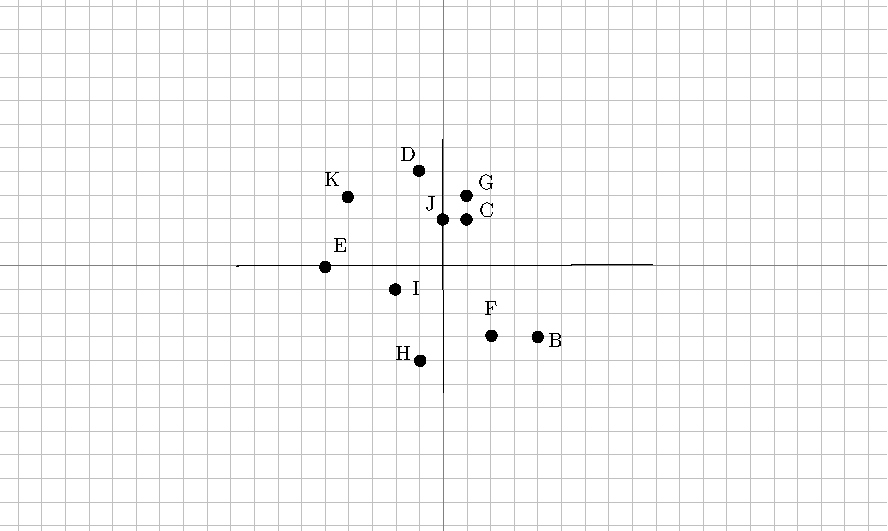
\includegraphics[scale=1,bb = 115 65 310 190, clip=true]{II_1_3bp-1.eps}
\end{multicols}

\

{\tmstrong{Plot each point.}}

2) L$(- 5, 5)$ \ \ \ \ \ \ K$(1, 0)$ \ \ \ \ \ \ \ \ J $(- 3, 4)$

\ \ \ \ I$(- 3, 0)$ \ \ \ \ \ \ \ H $(- 4, 2) \ \ \ \ $ G$(4, -2)$

\ \ \ \ F$(- 2, - 2)$ \ \ \ \ E $(3, - 2)$ \ \ \ \ D(0, 3)

\ \ \ \ C$(0, 4)$

\subsubsection{Graphing Lines from Points}\par

{\tmstrong{Sketch the graph of each line.}}

\begin{multicols}{2}
  1) $y = - \frac{1}{4} x - 3$
  
  3) $y = - \frac{5}{4} x - 4$
  
  5) $y = - 4 x + 2$
  
  7) $y = \frac{3}{2} x - 5$
  
  9) $y = - \frac{4}{5} x - 3$
  
  11) $x + 5 y = - 15$
  
  13) $4 x + y = 5$
  
  15) $2 x - y = 2$
  
  17) $x + y = - 1$
  
  19) $x - y = - 3$
  
  2) $y = x - 1$
  
  4) $y = - \frac{3}{5} x + 1$
  
  6) $y = \frac{5}{3} x + 4$
  
  8) $y = - x - 2$
  
  10) $y = \frac{1}{2} x$
  
  12) $8 x - y = 5$
  
  14) $3 x + 4 y = 16$
  
  16) $7 x + 3 y = - 12$
  
  18) $3 x + 4 y = 8$
  
  20) $9 x - y = - 4$
\end{multicols}

\pagebreak

\subsubsection{The Slope of a Line}\par

{\tmstrong{Find the slope of each line.}}
\label{lineargraphs1}
\begin{multicols}{2}
  1)\\
	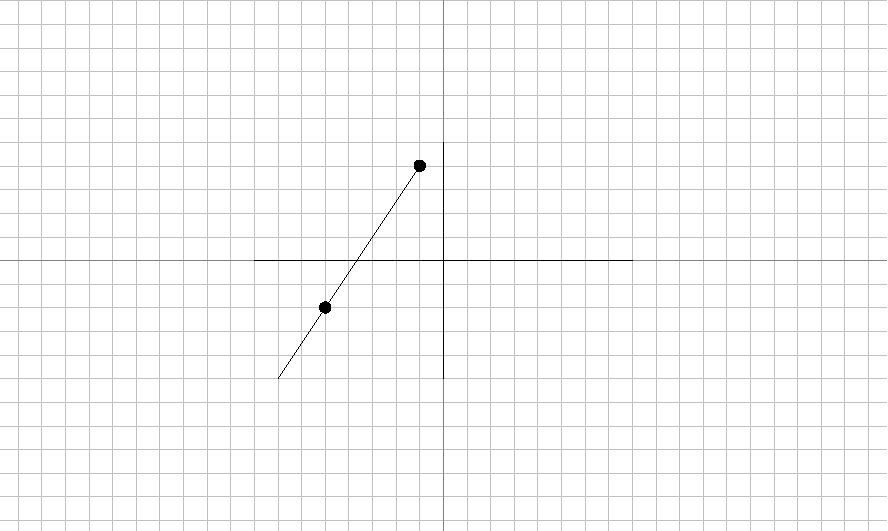
\includegraphics[scale=.8,bb = 115 65 310 190, clip=true]{II_1_3cp-1.eps}
  
  3)\\
	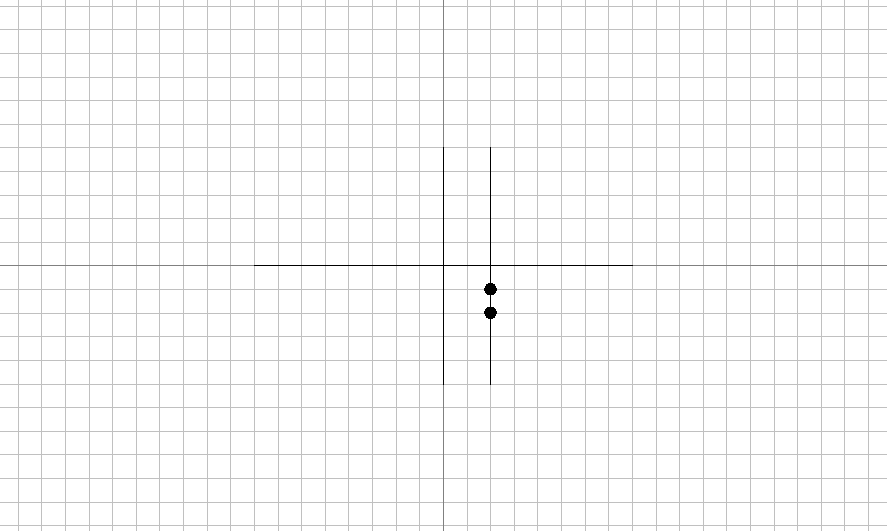
\includegraphics[scale=.8,bb = 115 65 310 190, clip=true]{II_1_3cp-2.eps}
  
  %5)\\
	%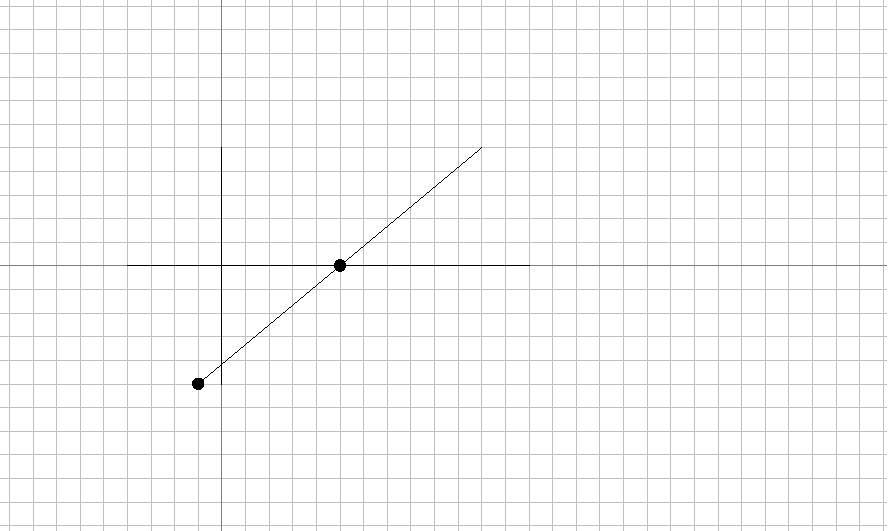
\includegraphics[scale=.8,bb = 115 65 310 190, clip=true]{II_1_3cp-3.eps}
  
%  7)\\
%	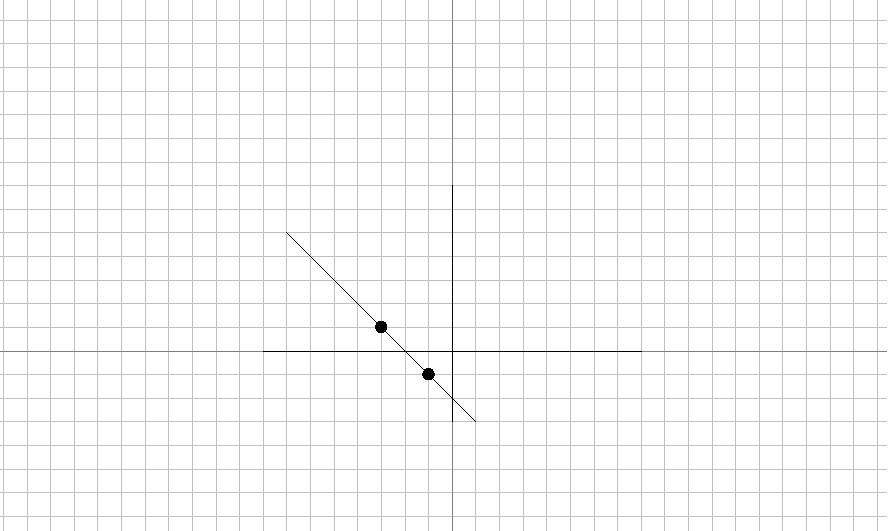
\includegraphics[scale=.8,bb = 115 65 310 190, clip=true]{II_1_3cp-4.eps}
  
%  \
  
  %2)\\
	%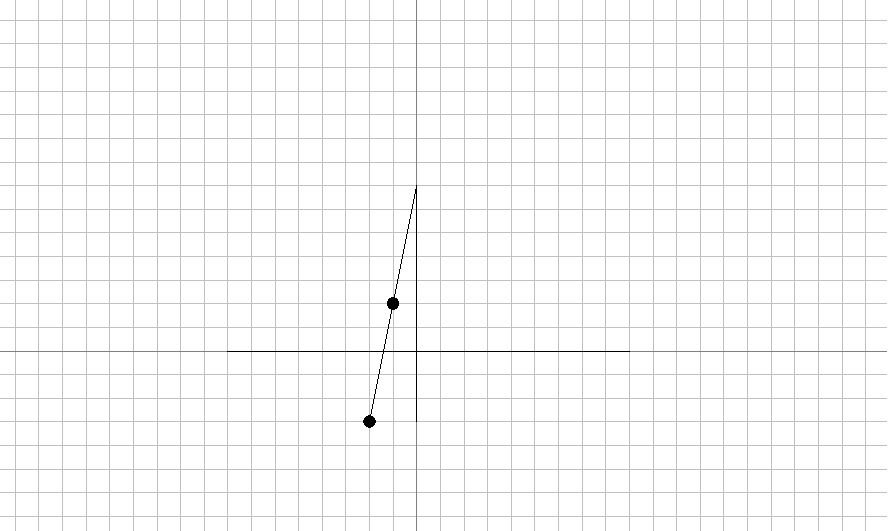
\includegraphics[scale=.8,bb = 115 65 310 190, clip=true]{II_1_3cp-5.eps}
  
  5)\\
	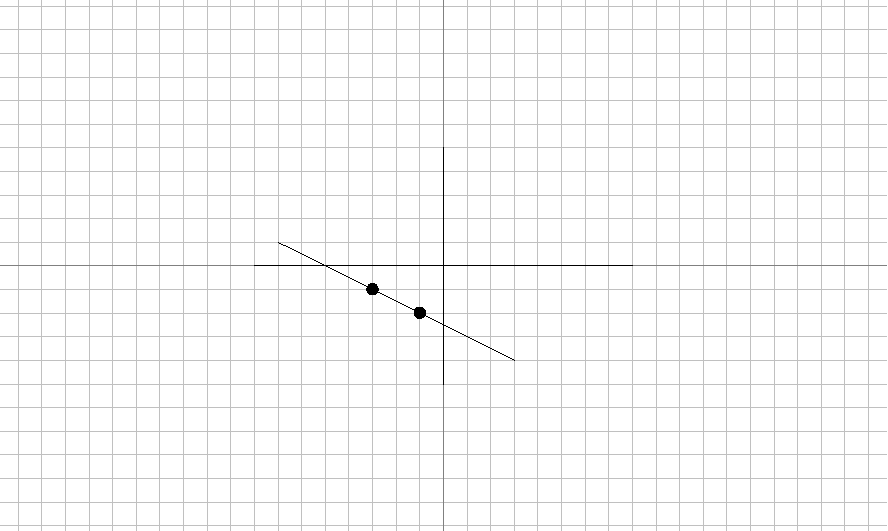
\includegraphics[scale=.8,bb = 115 65 310 190, clip=true]{II_1_3cp-6.eps}
  
  2)\\
	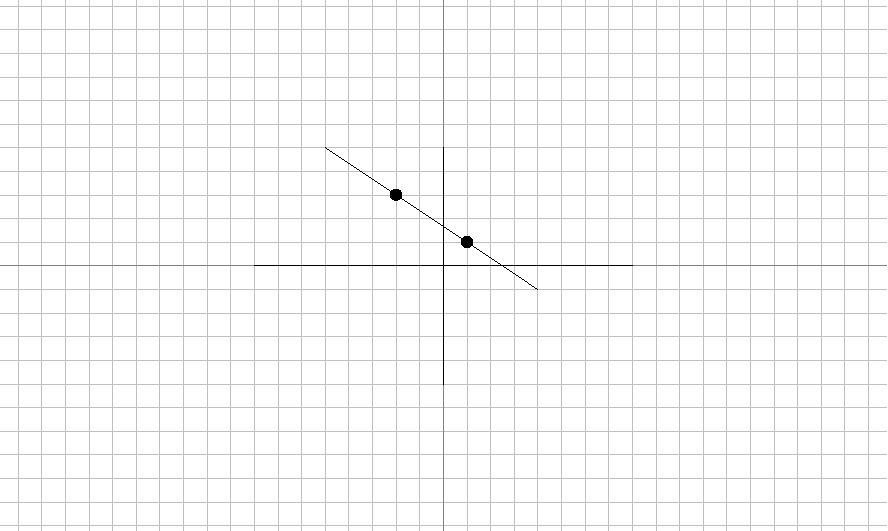
\includegraphics[scale=.8,bb = 115 65 310 190, clip=true]{II_1_3cp-7.eps}
  
%  8)\\
%	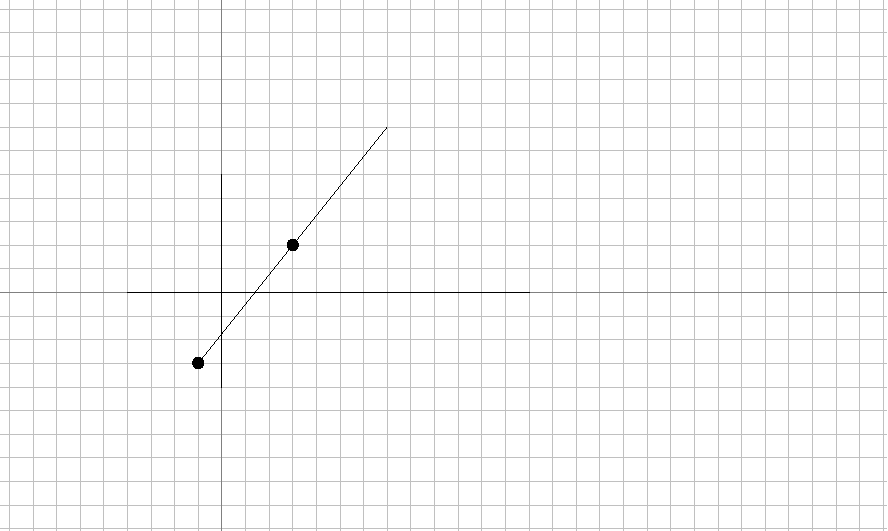
\includegraphics[scale=.8,bb = 115 65 310 190, clip=true]{II_1_3cp-8.eps}
  
  %{\pagebreak}
  
  4)\\
	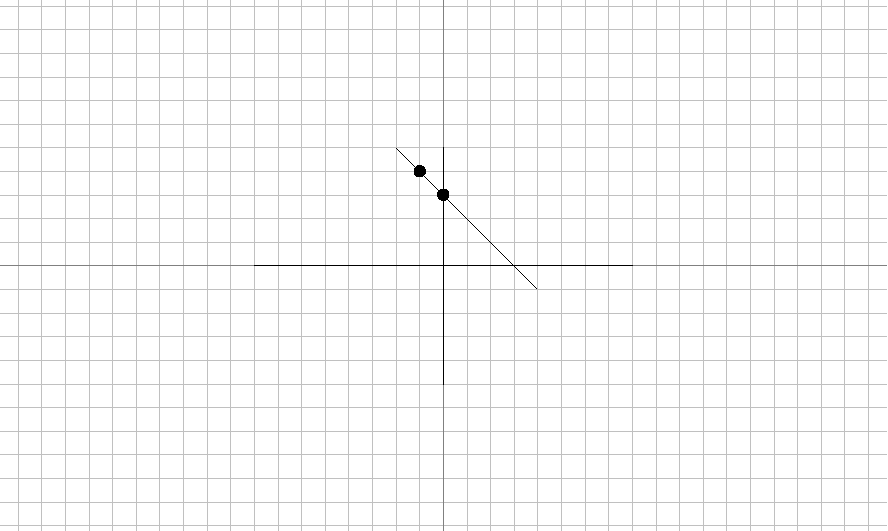
\includegraphics[scale=.8,bb = 115 65 310 190, clip=true]{II_1_3cp-9.eps}
  
  6)\\  
  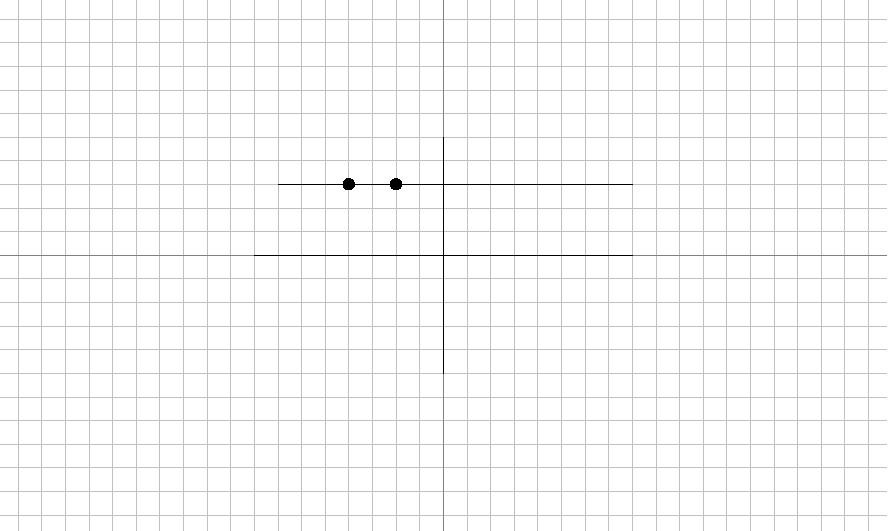
\includegraphics[scale=.8,bb = 115 65 310 190, clip=true]{II_1_3cp-10.eps}
\end{multicols}

\vspace{1in}
~

\pagebreak

{\tmstrong{Find the slope of the line through each pair of points.}}

\begin{multicols}{2}
  7) $(- 2, 10), (- 2, - 15)$
  
  9) $(- 15, 10), (16, - 7)$
  
  11) $(10, 18), (- 11, - 10)$
  
  13) $(- 16, - 14), (11, - 14)$
  
  15) $(- 4, 14), (- 16, 8)$
  
  17) $(12, - 19), (6, 14)$
  
  19) $(- 5, - 10), (- 5, 20)$
  
  21) $(- 17, 19), (10, - 7)$
  
  23) $(7, - 14), (- 8, - 9)$
  
  25) $(- 5, 7), (- 18, 14)$
  
  8) $(1, 2), (- 6, - 14)$
  
  10) $(13, - 2), (7, 7)$
  
  12) $(- 3, 6), (- 20, 13)$
  
  14) $(13, 15), (2, 10)$
  
  16) $(9, - 6), (- 7, - 7)$
  
  18) $(- 16, 2), (15, - 10)$
  
  20) $(8, 11), (- 3, - 13)$
  
  22) $(11, - 2), (1, 17)$
  
  24) $(- 18, - 5), (14, - 3)$
  
  26) $(19, 15), (5, 11)$
\end{multicols}

\

{\tmstrong{Find the value of x or y so that the line through the points has
the given slope.}}

\begin{multicols}{2}
  27) $(2, 6) \tmop{and} (x, 2) ; \tmop{slope} : \frac{4}{7}$
  
  29) $(- 3, - 2) \tmop{and} (x, 6) ; \tmop{slope} : - \frac{8}{5}$
  
  31) $(- 8, y) \tmop{and} (- 1, 1) ; \tmop{slope} : \frac{6}{7}$
  
  33) $(x, - 7) \tmop{and} (- 9, - 9) ; \tmop{slope} : \frac{2}{5}$
  
  35) $(x, 5) \tmop{and} (8, 0) ; \tmop{slope} : - \frac{5}{6}$
  
  28) $(8, y) \tmop{and} (- 2, 4) ; \tmop{slope} : - \frac{1}{5}$
  
  30) $(- 2, y) \tmop{and} (2, 4) ; \tmop{slope} : \frac{1}{4}$
  
  32) $(x, - 1) \tmop{and} (- 4, 6) ; \tmop{slope} : - \frac{7}{10}$
  
  34) $(2, - 5) \tmop{and} (3, y) ; \tmop{slope} : 6$
  
  36) $(6, 2) \tmop{and} (x, 6) ; \tmop{slope} : - \frac{4}{5}$
\end{multicols}

\vspace{2in}
~

\pagebreak

\subsection{The Two Forms of a Linear Equation}\par

	\subsubsection{Slope-Intercept Form}\par

{\tmstrong{Write the slope-intercept form of the equation of each line given
the slope and the y-intercept.}}

\begin{multicols}{2}
  1) Slope = 2, y-intercept = 5
  
  3) Slope = 1, y-intercept = $- 4$
  
  5) Slope = $- \frac{3}{4}$, y-intercept = $- 1$
  
  7) Slope = $\frac{1}{3}$, y-intercept = 1
  
  2) Slope = $- 6$, y-intercept = 4
  
  4) Slope = $- 1$, y-intercept = $- 2$
  
  6) Slope = $- \frac{1}{4}$, y-intercept = 3
  
  8) Slope = $\frac{2}{5}$, y-intercept = 5
\end{multicols}

{\tmstrong{Write the slope-intercept form of the equation of each line.}}

\begin{multicols}{2}
%  9)\\
%	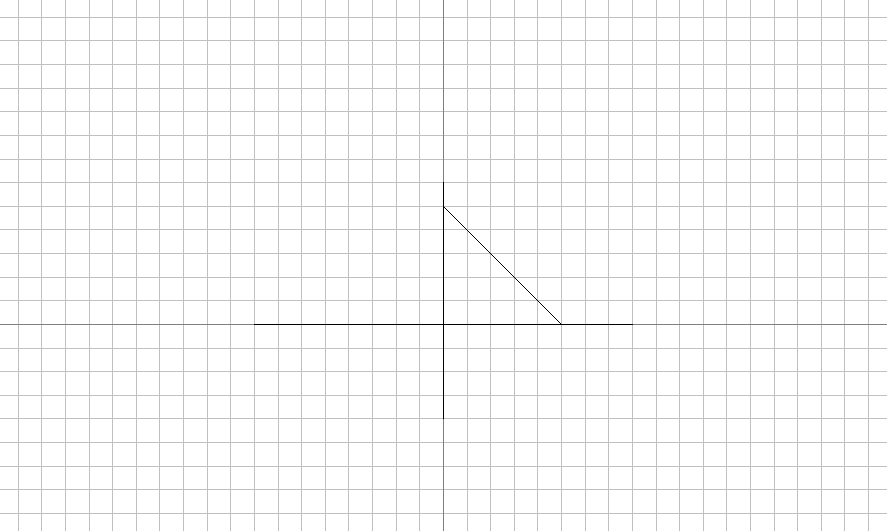
\includegraphics[scale=.7,bb = 115 65 310 190, clip=true]{II_1_4ap-1.eps}
  
  9)\\
	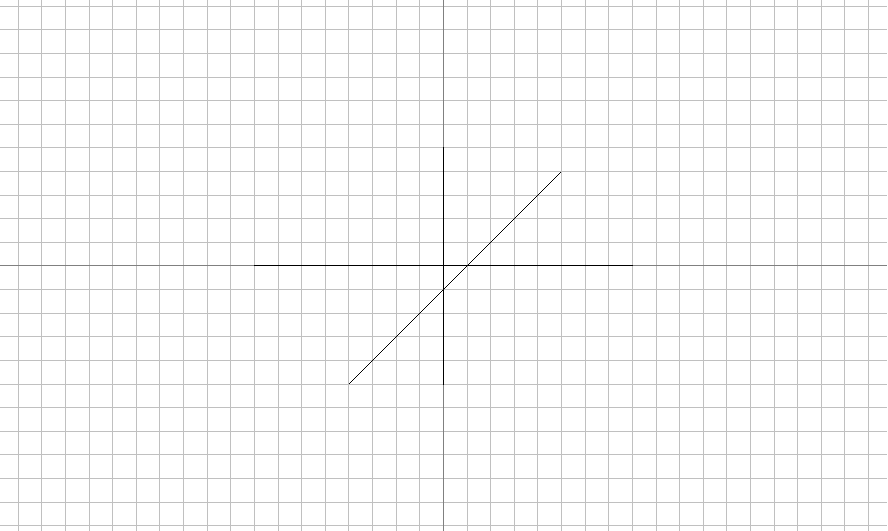
\includegraphics[scale=.7,bb = 115 65 310 190, clip=true]{II_1_4ap-2.eps}
  
  10)\\
	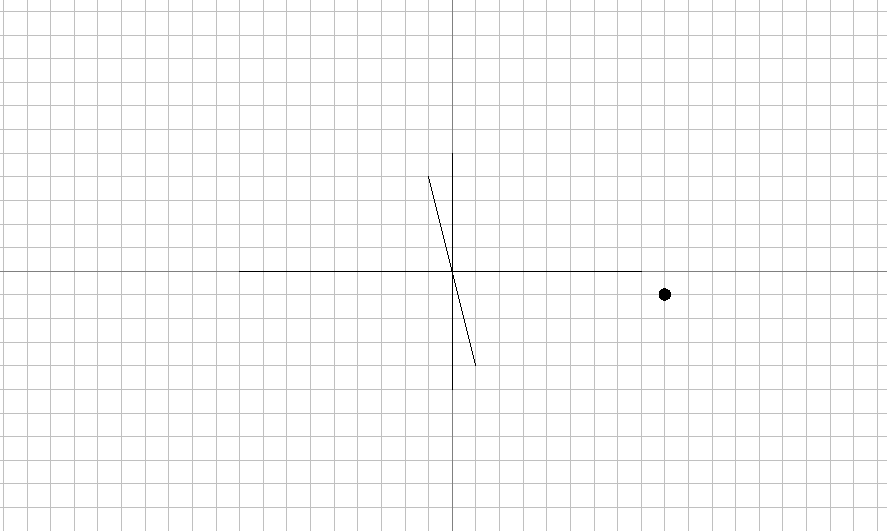
\includegraphics[scale=.7,bb = 115 65 310 190, clip=true]{II_1_4ap-3.eps}
  
 % 10)\\
%	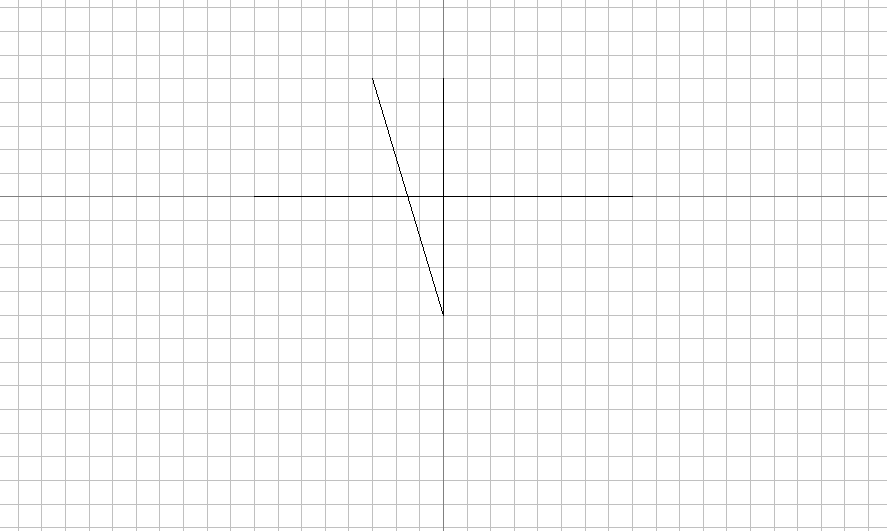
\includegraphics[scale=.7,bb = 115 65 310 190, clip=true]{II_1_4ap-4.eps}
  
 % 12)\\
%	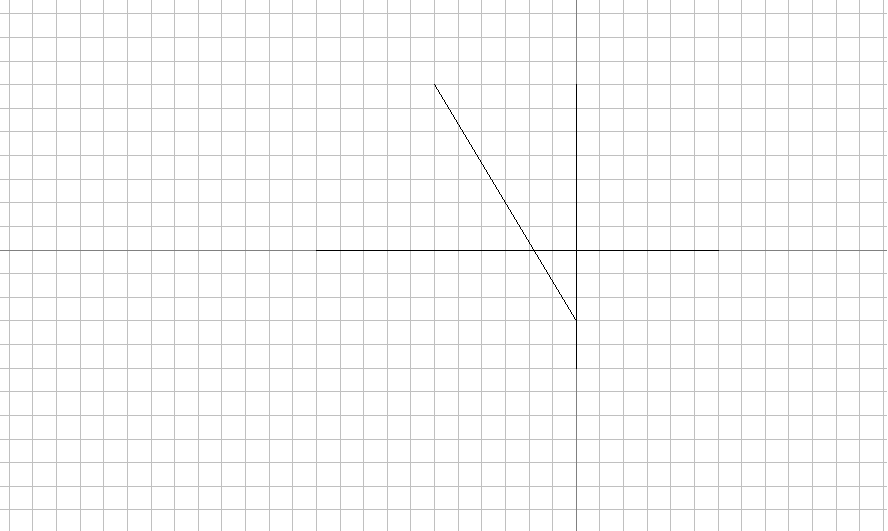
\includegraphics[scale=.7,bb = 115 65 310 190, clip=true]{II_1_4ap-5.eps}
  
 % 14)\\
%	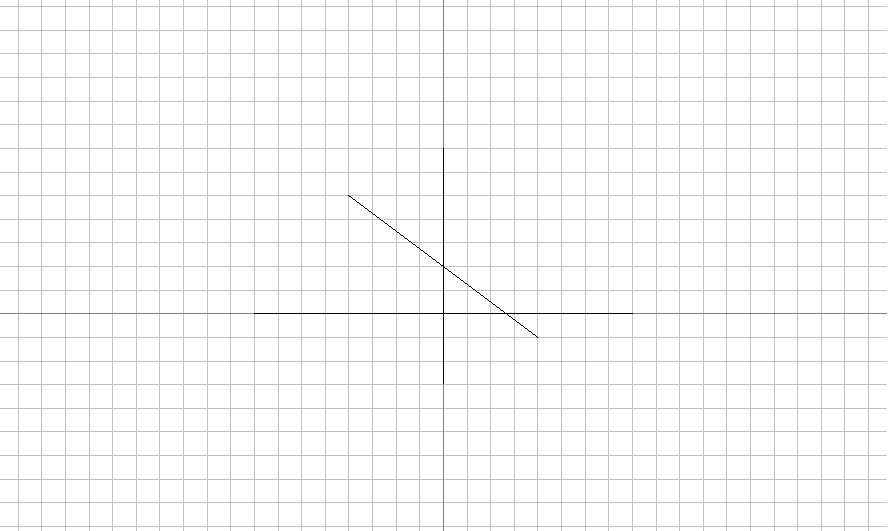
\includegraphics[scale=.7,bb = 115 65 310 190, clip=true]{II_1_4ap-6.eps}
\end{multicols}

%\pagebreak

{\tmstrong{Write each linear equation in slope-intercept form.}}

\begin{multicols}{2}
  11) $x + 10 y = - 37$
  
  13) $2 x + y = - 1$
  
  15) $7 x - 3 y = 24$
  
  17) $x = - 8$
  
  19) $y - 4 = - (x + 5)$
  
  21) $y - 4 = 4 (x - 1)$
  
  23) $y + 5 = - 4 (x - 2)$
  
  25) $y + 1 = - \frac{1}{2} (x - 4)$
  
  12) $x - 10 y = 3$
  
  14) $6 x - 11 y = - 70$
  
  16) $4 x + 7 y = 28$
  
  18) $x - 7 y = - 42$
  
  20) $y - 5 = \frac{5}{2} (x - 2)$
  
  22) $y - 3 = - \frac{2}{3} (x + 3)$
  
  24) $0 = x - 4$
  
  26) $y + 2 = \frac{6}{5} (x + 5)$
\end{multicols}

{\tmstrong{Sketch the graph of each line.}}
\label{lineargraphs2}
\begin{multicols}{2}
  27) $y = \frac{1}{3} x + 4$
  
  29) $y = \frac{6}{5} x - 5$
  
  31) $y = \frac{3}{2} x$
  
  33) $x - y + 3 = 0$
  
  35) $- y - 4 + 3 x = 0$
  
  37) $- 3 y = - 5 x + 9$
  
  28) $y = - \frac{1}{5} x - 4$
  
  30) $y = - \frac{3}{2} x - 1$
  
  32) $y = - \frac{3}{4} x + 1$
  
  34) $4 x + 5 = 5 y$
  
  36) $- 8 = 6 x - 2 y$
  
  38) $- 3 y = 3 - \frac{3}{2} x$
\end{multicols}

%\vspace{3in}
%~	

\pagebreak

	\subsubsection{Point-Slope Form}\par

{\tmstrong{Write the point-slope form of the equation of the line through the
given point with the given slope.}}

\begin{multicols}{2}
  1) $\tmop{through} (2, 3), \tmop{slope} = \tmop{undefined}$
  
  3) $\tmop{through} (2, 2), \tmop{slope} = \frac{1}{2}$
  
  5) $\tmop{through} (- 1, - 5), \tmop{slope} =$9
  
  7) $\tmop{through} (- 4, 1), \tmop{slope} = \frac{3}{4}$
  
  9) $\tmop{through} (0, - 2), \tmop{slope} = - 3$
  
  11) $\tmop{through} (0, - 5), \tmop{slope} = - \frac{1}{4}$
  
  13) $\tmop{through} (- 5, - 3), \tmop{slope} = \frac{1}{5}$
  
  15) $\tmop{through} (- 1, 4), \tmop{slope} = - \frac{5}{4}$
  
  2) $\tmop{through} (1, 2), \tmop{slope} =$undefined
  
  4) $\tmop{through} (2, 1), \tmop{slope} = - \frac{1}{2}$
  
  6) $\tmop{through} (2, - 2), \tmop{slope} = - 2$
  
  8) $\tmop{through} (4, - 3), \tmop{slope} = - 2$
  
  10) $\tmop{through} (- 1, 1), \tmop{slope} = 4$
  
  12) $\tmop{through} (0, 2), \tmop{slope} = - \frac{5}{4}$
  
  14) $\tmop{through} (- 1, - 4), \tmop{slope} = - \frac{2}{3}$
  
  16) $\tmop{through} (1, - 4), \tmop{slope} = - \frac{3}{2}$
\end{multicols}

\

{\tmstrong{Write the slope-intercept form of the equation of the line through
the given point with the given slope.}}

\begin{multicols}{2}
  17) through: $(- 1, - 5), \tmop{slope} = 2$
  
  19) through: $(5, - 1), \tmop{slope} = - \frac{3}{5}$
  
  21) through: $(- 4, 1), \tmop{slope} = \frac{1}{2}$
  
  23) through: $(4, - 2), \tmop{slope} = - \frac{3}{2}$
  
  25) through: $(- 5, - 3), \tmop{slope} = - \frac{2}{5}$
  
  27) through: $(2, - 2), \tmop{slope} = 1$
  
  29) through:$(- 3, 4)$, slope=undefined
  
  31) through: $(- 4, 2), \tmop{slope} = - \frac{1}{2}$
  
  18) through: $(2, - 2), \tmop{slope} = - 2$
  
  20) through: $(- 2, - 2), \tmop{slope} = - \frac{2}{3}$
  
  22) through: $(4, - 3), \tmop{slope} = - \frac{7}{4}$
  
  24) through: $(- 2, 0), \tmop{slope} = - \frac{5}{2}$
  
  26) through: $(3, 3), \tmop{slope} = \frac{7}{3}$
  
  28) through: $(- 4, - 3), \tmop{slope} =$0
  
  30) through: $(- 2, - 5), \tmop{slope} =$2
  
  32) through: $(5, 3), \tmop{slope} = \frac{6}{5}$
\end{multicols}

\

{\pagebreak}

{\tmstrong{Write the point-slope form of the equation of the line through the
given points.}}

\begin{multicols}{2}
  33) through: $(- 4, 3) \tmop{and} (- 3, 1)$
  
  35) through: $(5, 1) \tmop{and} (- 3, 0)$
  
  37) through: $(- 4, - 2) \tmop{and} (0, 4)$
  
  39) through: $(3, 5) \tmop{and} (- 5, 3)$
  
  41) through: $(3, - 3) \tmop{and} (- 4, 5)$
  
  34) through: $(1, 3) \tmop{and} (- 3, 3)$
  
  36) through: $(- 4, 5) \tmop{and} (4, 4)$
  
  38) through: $(- 4, 1) \tmop{and} (4, 4)$
  
  40) through: $(- 1, - 4) \tmop{and} (- 5, 0)$
  
  42) through: $(- 1, - 5) \tmop{and} (- 5, - 4)$
\end{multicols}

\

{\tmstrong{Write the slope-intercept form of the equation of the line through
the given points.}}

\begin{multicols}{2}
  43) through: $(- 5, 1) \tmop{and} (- 1, - 2)$
  
  45) through: $(- 5, 5) \tmop{and} (2, - 3)$
  
  47) through: $(4, 1) \tmop{and} (1, 4)$
  
  49) through: $(0, 2) \tmop{and} (5, - 3)$
  
  51) through: $(0, 3) \tmop{and} (- 1, - 1)$
  
  44) through: $(- 5, - 1) \tmop{and} (5, - 2)$
  
  46) through: $(1, - 1) \tmop{and} (- 5, - 4)$
  
  48) through: $(0, 1) \tmop{and} (- 3, 0)$
  
  50) through: $(0, 2) \tmop{and} (2, 4)$
  
  52) through: $(- 2, 0) \tmop{and} (5, 3)$
\end{multicols}

\vspace{2in}
~

\pagebreak

\subsection{Parallel and Perpendicular Lines}\par

{\tmstrong{Find the slope of a line parallel to each given line.}}

\begin{multicols}{2}
  1) $y = 2 x + 4$
  
  3) $y = 4 x - 5$
  
  5) $x - y = 4$
  
  7) $7 x + y = - 2$
  
  2) $y = - \frac{2}{3} x + 5$
  
  4) $y = - \frac{10}{3} x - 5$
  
  6) $6 x - 5 y = 20$
  
  8) $3 x + 4 y = - 8$
\end{multicols}

\

{\tmstrong{Find the slope of a line perpendicular to each given line.}}

\begin{multicols}{2}
  9) $x = 3$
  
  11) $y = - \frac{1}{3} x$
  
  13) $x - 3 y = - 6$
  
  15) $x + 2 y = 8$
  
  10) $y = - \frac{1}{2} x - 1$
  
  12) $y = \frac{4}{5} x$
  
  14) $3 x - y = - 3$
  
  16) $8 x - 3 y = - 9$
\end{multicols}

\

{\tmstrong{Write the point-slope form of the equation of the line
described.}}

17) $\tmop{through} : (2, 5), \tmop{parallel} \tmop{to} x = 0$

18) through: (5, 2), parallel to $y = \frac{7}{5} x + 4$

19) $\tmop{through} : (3, 4), \tmop{parallel} \tmop{to} y = \frac{9}{2} x - 5$

20) through: $(1, - 1), \tmop{parallel} \tmop{to} y = - \frac{3}{4} x + 3$

21) $\tmop{through} : (2, 3), \tmop{parallel} \tmop{to} y = \frac{7}{5} x + 4$

22) $\tmop{through} : (- 1, 3), \tmop{parallel} \tmop{to} y = - 3 x - 1$

23) $\tmop{through} : (4, 2), \tmop{parallel} \tmop{to} x = 0$

24) $\tmop{through} : (1, 4), \tmop{parallel} \tmop{to} y = \frac{7}{5} x + 2$

25) through: (1, $- 5), \tmop{perpendicular} \tmop{to} - x + y = 1$

26) $\tmop{through} : (1, - 2), \tmop{perpendicular} \tmop{to} - x + 2 y = 2$

27) $\tmop{through} : (5, 2), \tmop{perpendicular} \tmop{to} 5 x + y = - 3$

28) through: (1, 3), $\tmop{perpendicular} \tmop{to} - x + y = 1$

29) $\tmop{through} : (4, 2), \tmop{perpendicular} \tmop{to} - 4 x + y = 0$

30) through: $(- 3, - 5), \tmop{perpendicular} \tmop{to} 3 x + 7 y = 0$

31) $\tmop{through} : (2, - 2) \tmop{perpendicular} \tmop{to} 3 y - x = 0$

32) through: $(- 2, 5) . \tmop{perpendicular} \tmop{to} y - 2 x = 0$

\pagebreak

{\tmstrong{Write the slope-intercept form of the equation of the line
described.}}

33) $\tmop{through} : (4, - 3), \tmop{parallel} \tmop{to} y = - 2 x$

34) $\tmop{through} : (- 5, 2), \tmop{parallel} \tmop{to} y = \frac{3}{5} x$

35) $\tmop{through} : (- 3, 1), \tmop{parallel} \tmop{to} y = - \frac{4}{3} x
- 1$

36) $\tmop{through} : (- 4, 0), \tmop{parallel} \tmop{to} y = - \frac{5}{4} x
+ 4$

37) $\tmop{through} : (- 4, - 1), \tmop{parallel} \tmop{to} y = - \frac{1}{2}
x + 1$

38) $\tmop{through} : (2, 3), \tmop{parallel} \tmop{to} y = \frac{5}{2} x - 1$

39) $\tmop{through} : (- 2, - 1), \tmop{parallel} \tmop{to} y = - \frac{1}{2}
x - 2$

40) $\tmop{through} : (- 5, - 4), \tmop{parallel} \tmop{to} y = \frac{3}{5} x
- 2$

41) $\tmop{through} : (4, 3), \tmop{perpendicular} \tmop{to} x + y = - 1$

42) $\tmop{through} : (- 3, - 5), \tmop{perpendicular} \tmop{to} x + 2 y = -
4$

43) $\tmop{through} : (5, 2), \tmop{perpendicular} \tmop{to} x = 0$

44) $\tmop{through} : (5, - 1), \tmop{perpendicular} \tmop{to} - 5 x + 2 y =
10$

45) $\tmop{through} : (- 2, 5), \tmop{perpendicular} \tmop{to} - x + y = - 2$

46) $\tmop{through} : (2, - 3), \tmop{perpendicular} \tmop{to} - 2 x + 5 y = -
10$

47) $\tmop{through} : (4, - 3), \tmop{perpendicular} \tmop{to} - x + 2 y = -
6$

48) $\tmop{through} : (- 4, 1), \tmop{perpendicular} \tmop{to} 4 x + 3 y = -
9$

\vspace{3in}
~

\pagebreak

\subsection{Applications}\par

	\subsubsection{Numbers and Geometry}\par

{\tmstrong{Solve.}}

1. When five is added to three more than a certain number, the result is 19.  What is the number?

2. If five is subtracted from three times a certain number, the result is
$10$. What is the number?

3. When 18 is subtracted from six times a certain number, the result is $-
42$. What is the number?

4. A certain number added twice to itself equals 96. What is the number?

5. A number plus itself, plus twice itself, plus 4 times itself, is equal to
$- 104$. What is the number?

6. Sixty more than nine times a number is the same as two less than ten times
the number. What is the number?

7. Eleven less than seven times a number is five more than six times the
number. Find the number.

8. Fourteen less than eight times a number is three more than four times the number. What is the number?

9. The sum of three consecutive integers is 108. What are the integers?

10. The sum of three consecutive integers is $- 126$. What are the integers?

11. Find three consecutive integers such that the sum of the first, twice the
second, and three times the third is $- 76$.

12. The sum of two consecutive even integers is 106. What are the integers?

13. The sum of three consecutive odd integers is 189. What are the integers?

14. The sum of three consecutive odd integers is 255. What are the integers?

15. Find three consecutive odd integers such that the sum of the first, two
times the second, and three times the third is 70.

16. The second angle of a triangle is the same size as the first angle. The
third angle is 12 degrees larger than the first angle. How
large are the angles?

17. Two angles of a triangle are the same size. The third angle is 12 degrees
smaller than the first angle. Find the measure of the
angles.

18. Two angles of a triangle are the same size. The third angle is 3 times as
large as the first. How large are the angles?

19. The third angle of a triangle is the same size as the first. The second
angle is 4 times the third. Find the measure of the angles.

\pagebreak

20. The second angle of a triangle is 3 times as large as the first angle. The
third angle is 30 degrees more than the first angle. Find the
measure of the angles.

21. The second angle of a triangle is twice as large as the first. The measure
of the third angle is 20 degrees greater than the first. How
large are the angles?

22. The second angle of a triangle is three times as large as the first. The
measure of the third angle is 40 degrees greater than that of the
first angle. How large are the three angles?

23. The second angle of a triangle is five times as large as the first. The
measure of the third angle is 12 degrees greater than that of
the first angle. How large are the angles?

24. The second angle of a triangle is three times the first, and the third is
12 degrees less than twice the first. Find the
measures of the angles.

25. The second angle of a triangle is four times the first and the third is 5
degrees more than twice the first. Find the measures of the angles.

26. The perimeter of a rectangle is 150 cm. The length is 15 cm greater than
the width. Find the dimensions.

27. The perimeter of a rectangle is 304 cm. The length is 40 cm longer than
the width. Find the length and width.

28. The perimeter of a rectangle is 152 meters. The width is 22 meters less
than the length. Find the length and width.

29. The perimeter of a rectangle is 280 meters. The width is 26 meters less
than the length. Find the length and width.

30. The perimeter of a college basketball court is 96 meters and the length is
14 meters more than the width. What are the dimensions?

31. A mountain cabin on 1 acre of land costs $\$30,000$. If the land
cost 4 times as much as the cabin, what was the cost of each?

32. A horse and a saddle cost $\$5000$. If the horse cost 4 times as
much as the saddle, what was the cost of each?

33. A bicycle and a bicycle helmet cost $\$240$. How much did each
cost, if the bicycle cost 5 times as much as the helmet?

34. Of 240 stamps that Harry and his sister collected, Harry collected 3 times
as many as his sisters. How many did each collect?

35. If Mr. Brown and his son together had $\$220$, and Mr. Brown had
10 times as much as his son, how much money had each?

36. In a room containing 45 students there were twice as many girls as boys.
How many of each were there?

37. Aaron had 7 times as many sheep as Beth, and both together had 608. How many sheep had each?

\pagebreak

38. A man bought a cow and a calf for $\$990$, paying 8 times as much
for the cow as for the calf. What was the cost of each?

39. Jamal and Moshe began a business with a capital of $\$7500$. If
Jamal furnished half as much capital as
Moshe, how much did each furnish?

40. A lab technician cuts a 12 inch piece of tubing into two pieces in such a
way that one piece is 2 times longer than the other.

41. A 6 ft board is cut into two pieces, one twice as long as the other. How
long are the pieces?

42. An eight ft board is cut into two pieces. One piece is 2 ft longer than
the other. How long are the pieces?

43. An electrician cuts a 30 ft piece of wire into two pieces. One piece is 2
ft longer than the other. How long are the pieces?

44. The total cost for tuition plus room and board at State University is
$\$2,584$. Tuition costs $\$704$ more than
room and board. What is the tuition fee?

45. The cost of a private pilot course is $\$1,275$. The flight
portion costs $\$625$ more than the groung
school portion. What is the cost of each?

\vspace{4in}
~

\pagebreak

	\subsubsection{Age Problems}\par

1. A boy is 10 years older than his brother. In 4 years he will be twice as
old as his brother. Find the present age of each.

2. A father is 4 times as old as his son. In 20 years the father will be
twice as old as his son. Find the present age of each.

3. Pat is 20 years older than his son James. In two years Pat will be twice as
old as James. How old are they now?

4. Diane is 23 years older than her daughter Amy. In 6 years Diane will be
twice as old as Amy. How old are they now?

5. Fred is 4 years older than Barney. Five years ago the sum of their ages was
48. How old are they now?

6. John is four times as old as Martha. Five years ago the sum of their ages
was 50. How old are they now?

7. Tim is 5 years older than JoAnn. Six years from now the sum of their ages
will be 79. How old are they now?

8. Jack is twice as old as Lacy. In three years the sum of their ages will be
54. How old are they now?

9. The sum of the ages of John and Mary is 32. Four years ago, John was twice
as old as Mary. Find the present age of each.

10. The sum of the ages of a father and son is 56. Four years ago the father
was 3 times as old as the son. Find the present age of each.

11. The sum of the ages of a china plate and a glass plate is 16 years. Four
years ago the china plate was three times the age of the glass
plate. Find the present age of each plate.

12. The sum of the ages of a wood plaque and a bronze plaque is 20 years. Four
years ago, the bronze plaque was one-half the age of the wood
plaque. Find the present age of each plaque.

13. Adam is now 34 years old, and Bryce is 4 years old. In how many years will Adam be twice as old as Bryce?

14. A man's age is 36 and that of his daughter is 3 years. In how many years
will the man be 4 times as old as his daughter?

15. An Oriental rug is 52 years old and a Persian rug is 16 years old. How
many years ago was the Oriental rug four times as old as the
Persian Rug?

16. A log cabin quilt is 24 years old and a friendship quilt is 6 years old.
In how may years will the log cabin quilt be three times as old
as the friendship quilt?

17. The age of the older of two boys is twice that of the younger; 5 years ago
it was three times that of the younger. Find the age of
each.

18. A pitcher is 30 years old, and a vase is 22 years old. How many years ago
was the pitcher twice as old as the vase?

19. Marge is twice as old as Consuelo. The sum of their ages seven years ago
was 13. How old are they now?

20. The sum of Jason and Mandy's age is 35. Ten years ago Jason was double Mandy's age. How old are they now?

21. A silver coin is 28 years older than a bronze coin. In 6 years, the silver
coin will be twice as old as the bronze coin. Find the
present age of each coin.

22. A sofa is 12 years old and a table is 36 years old. In how many years will
the table be twice as old as the sofa?

23. A limestone statue is 56 years older than a marble statue. In 12 years,
the limestone will be three times as old as the marble
statue. Find the present age of the statues.

24. A pewter bowl is 8 years old, and a silver bowl is 22 years old. In how
many years will the silver bowl be twice the age of the pewter
bowl?

25. Brandon is 9 years older than Ronda. In four years the sum of their ages
will be 91. How old are they now?

26. A kerosene lamp is 95 years old, and an electric lamp is 55 years old. How
many years ago was the kerosene lamp twice the age of the
electric lamp?

27. A father is three times as old as his son, and his daughter is 3 years
younger than the son. If the sum of their ages 3 years ago
was 63 years, find the present age of the father.

28. The sum of Clyde and Wendy's age is 64. In four years, Wendy will be three
times as old as Clyde. How old are they now?

29. The sum of the ages of two ships is 12 years. Two years ago, the age of
the older ship was three times the age of the newer ship.
Find the present age of each ship.

30. Chelsea's age is double Daniel's age. Eight years ago the sum of their
ages was 32. How old are they now?

31. Ann is eighteen years older than her son. One year ago, she was three
times as old as her son. How old are they now?

32. The sum of the ages of Kristen and Ben is 32. Four years ago Kristen was twice as old as Ben. How old are they both now?

33. A mosaic is 74 years older than the engraving. Thirty years ago, the
mosaic was three times as old as the engraving. Find the
present age of each.

34. The sum of the ages of Elli and Dan is 56. Four years ago Elli was 3 times
as old as Dan. How old are they now?

35. A wool tapestry is 32 years older than a linen tapestry. Twenty years ago,
the wool tapestry was twice as old as the linen tapestry. Find the
present age of each.

36. Carolyn's age is triple her daughter's age. In eight years the sum of
their ages will be 72. How old are they now?

37. Nicole is 26 years old. Emma is 2 years old. In how many years will Nicole
be triple Emma's age?

38. The sum of the ages of two children is 16 years. Four years ago, the age
of the older child was three times the age of the younger child.
Find the present age of each child.

39. Mike is 4 years older than Ron. In two years, the sum of their ages will
be 84. How old are they now?

40. A marble bust is 25 years old, and a terra-cotta bust is 85 years old. In
how many years will the terra-cotta bust be three times as old
as the marble bust?

\vspace{4in}
~


\pagebreak

	\subsubsection{Distance, Rate and Time}\par

1. A is 60 miles from B. An automobile at A starts for B at the rate of 20
miles an hour at the same time that an automobile at B starts
for A at the rate of 25 miles an hour. How long will it be
before the automobiles meet?

2. Two automobiles are 276 miles apart and start at the same time to travel toward each other. They travel at rates differing by 5
miles per hour. If they meet after 6 hours, find the rate of
each.

3. Two trains travel toward each other from points which are 195 miles apart.
They travel at rate of 25 and 40 miles an hour respectively.
If they start at the same time, how soon will they meet?

4. A and B start toward each other at the same time from points 150 miles
apart. If A went at the rate of 20 miles an hour, at what rate must B
travel if they meet in 5 hours?

5. A passenger and a freight train start toward each other at the same time
from two points 300 miles apart. If the rate of the passenger train
exceeds the rate of the freight train by 15 miles per hour, and
they meet after 4 hours, what must the rate of each be?

6. Two automobiles started at the same time from a point, but traveled in opposite directions. Their rates were 25 and 35 miles
per hour respectively. After how many hours were they 180
miles apart?

7. A man having ten hours at his disposal made an excursion, riding out at the
rate of 10 miles an hour and returning on foot, at the rate of
3 miles an hour. Find the distance he rode.

8. A man walks at the rate of 4 miles per hour. How far can he walk into the country and ride back on a trolley that travels at the rate
of 20 miles per hour, if he must be back home 3 hours from the time he
started?

9. A boy rides away from home in an automobile at the rate of 28 miles an hour
and walks back at the rate of 4 miles an hour. The round trip
requires 2 hours. How far does he ride?

10. A motorboat leaves a harbor and travels at an average speed of 15 mph toward an island. The average speed on the return trip
was 10 mph. How far was the island from the harbor if the total
trip took 5 hours?

11. A family drove to a resort at an average speed of 30 mph and later
returned over the same road at an average speed of 50 mph.
Find the distance to the resort if the total driving time was
8 hours.

12. As part of his flight training, a student pilot was required to fly to an
airport and then return. The average speed to the airport was 90
mph, and the average speed returning was 120 mph.
Find the distance between the two airports if the total
flying time was 7 hours.

13. A, who travels 4 miles an hour starts from a certain place 2 hours in
advance of B, who travels 5 miles an hour in the same direction.
How many hours must B travel to overtake A?

14. A man travels 5 miles an hour. After traveling for 6 hours another man
starts at the same place, following at the rate of 8 miles an hour.
When will the second man overtake the first?

15. A motorboat leaves a harbor and travels at an average speed of 8 mph
toward a small island. Two hours later a cabin cruiser leaves the
same harbor and travels at an average speed of 16 mph
toward the same island. In how many hours after the cabin
cruiser leaves will the cabin cruiser be alongside the motorboat?

16. A long distance runner started on a course running at an average speed of
6 mph. One hour later, a second runner began the same course
at an average speed of 8 mph. How long after the second
runner started will the second runner overtake the first
runner?

17. A car traveling at 48 mph overtakes a cyclist who, riding at 12 mph, has
had a 3 hour head start. How far from the starting point does
the car overtake the cyclist?

18. A jet plane traveling at 600 mph overtakes a propeller-driven plane which
has had a 2 hour head start. The propeller-driven plane is
traveling at 200 mph. How far from the starting point does the
jet overtake the propeller-driven plane?

19. Two men are traveling in opposite directions at the rate of 20 and 30
miles an hour at the same time and from the same place. In how
many hours will they be 300 miles apart?

20. Running at an average rate of 8 m/s, a sprinter ran to the end of a track
and then jogged back to the starting point at an average rate of
3 m/s. The sprinter took 55 s to run to the end of
the track and jog back. Find the length of the
track.

21. A motorboat leaves a harbor and travels at an average speed of 18 mph to
an island. The average speed on the return trip was 12 mph. How
far was the island from the harbor if the total trip took
5 h?

22. A motorboat leaves a harbor and travels at an average speed of 9 mph
toward a small island. Two hours later a cabin cruiser leaves the
same harbor and travels at an average speed of 18 mph
toward the same island. In how many hours after the cabin
cruiser leaves will the cabin cruiser be alongside the motorboat?

\pagebreak

23. A jet plane traveling at 570 mph overtakes a propeller-driven plane that
has had a 2 h head start. The propeller-driven plane is
traveling at 190 mph. How far from the starting point
does the jet overtake the propeller-driven plane?

24. Two trains start at the same time from the same place and travel in
opposite directions. If the rate of one is 6 miles per hour more
than the rate of the other and they are 168 miles apart
at the end of 4 hours, what is the rate of each?

25. As part of flight training, a student pilot was required to fly to an
airport and then return. The average speed on the way to the
airport was 100 mph, and the average speed returning was 150
mph. Find the distance between the two airports if the total
flight time was 5 h.

26. Two cyclists start from the same point and ride in opposite directions.
One cyclist rides twice as fast as the other. In three
hours they are 72 miles apart. Find the rate of each cyclist.

27. A car traveling at 56 mph overtakes a cyclist who, riding at 14 mph, has
had a 3 h head start. How far from the starting point does the
car overtake the cyclist?

28. Two small planes start from the same point and fly in opposite directions.
The first plan is flying 25 mph slower than the second
plane. In two hours the planes are 430 miles apart. Find
the rate of each plane.

29. A bus traveling at a rate of 60 mph overtakes a car traveling at a rate of
45 mph. If the car had a 1 h head start, how far from the
starting point does the bus overtake the car?

30. Two small planes start from the same point and fly in opposite directions.
The first plane is flying 25 mph slower than the second
plane. In 2 h, the planes are 470 mi apart. Find the
rate of each plane.

31. A truck leaves a depot at 11 A.M. and travels at a speed of 45 mph. At
noon, a van leaves the same place and travels the same route at a
speed of 65 mph. At what time does the van overtake the truck?

32. A family drove to a resort at an average speed of 25 mph and later
returned over the same road at an average speed of 40 mph.
Find the distance to the resort if the total driving time was
13 h.

33. Three campers left their campsite by canoe and paddled downstream at an average rate of 10 mph. They then turned around and paddled
back upstream at an average rate of 5 mph
to return to their campsite. How long did it take the campers
to canoe downstream if the total trip took 1 hr?

\pagebreak

34. A motorcycle breaks down and the rider has to walk the rest of the way to
work. The motorcycle was being driven at 45 mph, and the
rider walks at a speed of 6 mph. The distance from home to
work is 25 miles, and the total time for the trip was 2
hours. How far did the motorcycle go before if broke down?

35. A student walks and jogs to college each day. The student averages 5 km/hr
walking and 9 km/hr jogging. The distance from home to college
is 8 km, and the student makes the trip in one hour. How
far does the student jog?

36. On a 130 mi trip, a car traveled at an average speed of 55 mph and then reduced its speed to 40 mph for the remainder of the
trip. The trip took a total of 2.5 h. For how long did the
car travel at 40 mph?

37. On a 220 mi trip, a car traveled at an average speed of 50 mph and then reduced its average speed to 35 mph for the remainder
of the trip. The trip took a total of 5 h. How long did the
car travel at each speed?

38. An executive drove from home at an average speed of 40 mph to an airport where a helicopter was waiting. The executive boarded the
helicopter and flew to the corporate offices at and
average speed of 60 mph. The entire distance was 150
mi. The entire trip took 3 h. Find the distance from the airport to the corporate offices.

\vspace{3in}
~

\pagebreak

\subsection{Linear Inequalities and Sign Diagrams}\par

{\tmstrong{Draw a graph for each inequality and provide interval notation.}}

\begin{multicols}{2}
  1) $n > - 5$
  
  3) $- 2 \geq k$
  
  5) $5 \geq x$
  
  2) $n > 4$
  
  4) $1 \geq k$
  
  6) $- 5 < x$
\end{multicols}

\

%{\tmstrong{Write an inequality for each graph.}}

%\begin{multicols}{2}
%  7)
  
%  \resizebox{391px}{55px}{\includegraphics{Inequalities - graph and solve -
%  problem set-1.eps}}
  
%  8)
  
%  \resizebox{391px}{55px}{\includegraphics{Inequalities - graph and solve -
%  problem set-2.eps}}
  
%  9)
  
%  \resizebox{391px}{55px}{\includegraphics{Inequalities - graph and solve -
%  problem set-3.eps}}
  
%  10)
  
%  \resizebox{391px}{55px}{\includegraphics{Inequalities - graph and solve -
%  problem set-4.eps}}
  
%  11)
  
%  \resizebox{391px}{55px}{\includegraphics{Inequalities - graph and solve -
%  problem set-5.eps}}
  
%  12)
  
%  \resizebox{391px}{55px}{\includegraphics{Inequalities - graph and solve -
%  problem set-6.eps}}
%\end{multicols}

{\tmstrong{Solve each inequality, graph each solution, and provide interval
notation.}}

\begin{multicols}{2}
  7) $\frac{x}{11} \geq 10$
  
  9) $2 + r < 3$
  
  11) $8 + \frac{n}{3} \geq 6$
  
  13) $2 > \frac{a - 2}{5}$
  
  15) $- 47 \geq 8 - 5 x$
  
  17) $- 2 (3 + k) < - 44$
  
  19) $18 < - 2 (- 8 + p)$
  
  21) $24 \geq - 6 (m - 6)$
  
  23) $- r - 5 (r - 6) < - 18$
  
  25) $24 + 4 b < 4 (1 + 6 b)$
  
  27) $- 5 v - 5 < - 5 (4 v + 1)$
  
  29) $4 + 2 (a + 5) < - 2 (- a - 4)$
  
  31) $- (k - 2) > - k - 20$
  
  8) $- 2 \leq \frac{n}{13}$
  
  10) $\frac{m}{5} \leq - \frac{6}{5}$
  
  12) $11 > 8 + \frac{x}{2}$
  
  14) $\frac{v - 9}{- 4} \leq 2$
  
  16) $\frac{6 + x}{12} \leq - 1$
  
  18) $- 7 n - 10 \geq 60$
  
  20) $5 \geq \frac{x}{5} + 1$
  
  22) $- 8 (n - 5) \geq 0$
  
  24) $- 60 \geq - 4 (- 6 x - 3)$
  
  26) $- 8 (2 - 2 n) \geq - 16 + n$
  
  28) $- 36 + 6 x > - 8 (x + 2) + 4 x$
  
  30) $3 (n + 3) + 7 (8 - 8 n) < 5 n + 5 + 2$
  
  32) $- (4 - 5 p) + 3 \geq - 2 (8 - 5 p)$ 
\end{multicols}

{\tmstrong{Construct a sign diagram for each of following graphs/linear equations referenced below.}}\pp

33)-38): Graphs (1) through (6) on page \pageref{lineargraphs1}.\pp

39)-50): Linear equations (27) through (38) on page \pageref{lineargraphs2}.\pp

%\vspace{2in}
%~

\pagebreak

\subsection{Compound and Absolute Value Inequalities}\par

\subsubsection{Compound Inequalities}\par

{\tmstrong{Solve each compound inequality, graph its solution, and provide interval notation.}}

\begin{multicols}{2}
  1) $\frac{n}{3} \leq - 3 \tmop{~or~} - 5 n \leq - 10$
  
  3) $x + 7 \geq 12 \tmop{~or~} 9 x < - 45$
  
  5) $x - 6 < - 13 \tmop{~or~} 6 x \leq - 60$
  
  7) $\frac{v}{8} > - 1 \tmop{~and~} v - 2 < 1$
  
  9) $- 8 + b < - 3 \tmop{~and~} 4 b < 20$
  
  11) $a + 10 \geq 3 \tmop{~and~} 8 a \leq 48$
  
  13) $3 \leq 9 + x \leq 7$
  
  15) $11 < 8 + k \leq 12$
  
  17) $- 3 < x - 1 < 1$
  
  19) $- 4 < 8 - 3 m \leq 11$
  
  21) $- 22 \leq 2 n - 10 \leq - 16$
  
  2) $6 m \geq - 24 \tmop{~or~} m - 7 < - 12$
  
  4) $10 r > 0 \tmop{~or~} r - 5 < - 12$
  
  6) $9 + n < 2 \tmop{~or~} 5 n > 40$
  
  8) $- 9 x < 63 \tmop{~and~} \frac{x}{4} < 1$
  
  10) $- 6 n \leq 12 \tmop{~and~} \frac{n}{3} \leq 2$
  
  12) $- 6 + v \geq 0 \tmop{~and~} 2 v > 4$
  
  14) $0 \geq \frac{x}{9} \geq - 1$
  
  16) $- 11 \leq n - 9 \leq - 5$
  
  18) $1 \leq \frac{p}{8} \leq 0$
  
  20) $3 + 7 r > 59 \tmop{~or~} - 6 r - 3 > 33$
  
  22) $- 6 - 8 x \geq - 6 \tmop{~or~} 2 + 10 x > 82$
  
\end{multicols}

  23) $- 5 b + 10 \leq 30 \tmop{~and~} 7 b + 2 \leq - 40$

  24) $n + 10 \geq 15 \tmop{~or~} 4 n - 5 < - 1$

	25) $3 x - 9 < 2 x + 10 \tmop{~and~} 5 + 7 x \leq 10 x - 10$
  	
  26) $4 n + 8 < 3 n - 6 \tmop{~or~} 10 n - 8 \geq 9 + 9 n$

  27) $- 8 - 6 v \leq 8 - 8 v \tmop{~and~} 7 v + 9 \leq 6 + 10 v$
  
  28) $5 - 2 a \geq 2 a + 1 \tmop{~or~} 10 a - 10 \geq 9 a + 9$
  
  29) $1 + 5 k \leq 7 k - 3 \tmop{~or~} k - 10 > 2 k + 10$
  
  30) $8 - 10 r \leq 8 + 4 r \tmop{~or~} - 6 + 8 r < 2 + 8 r$

  31) $2 x + 9 \geq 10 x + 1 \tmop{~and~} 3 x - 2 < 7 x + 2$

  32) $- 9 m + 2 < - 10 - 6 m \tmop{~or~} - m + 5 \geq 10 + 4 m$
  
\vspace{2in}
~

\pagebreak

\subsubsection{Absolute Value Inequalities}\par

{\tmstrong{Solve each inequality, graph its solution, and provide interval
notation.}}

\begin{multicols}{2}
  1) $| x | < 3$
  
  3) $| 2 x| < 6$
  
  5) $| x - 2| < 6$
  
  7) $|x - 7| < 3$
  
  9) $|3x - 2| < 9$
  
  11) $1 + 2 |x - 1| \leq 9$
  
  13) $6 - |2x - 5| \geq 3$
  
  15) $|3x| > 5$
  
  17) $| x - 3| \geq 3$
  
  19) $| 3 x - 5| \geq 3$
  
  21) $4 + 3 |x - 1| \geq 10$
  
  23) $3 - 2 |x - 5| \leq - 15$
  
  25) $- 2 - 3 |4 - 2 x| \geq - 8$
  
  27) $4 - 5| - 2 x - 7| < - 1$
  
  29) $3 - 2 |4x - 5| \geq 1$
  
  31) $- 5 - 2 |3x - 6| < - 8$
  
  33) $4 - 4| - 2 x + 6| > - 4$
  
  35) $| - 10 + x | \geq 8$
  
  2) $| x | \leq 8$
  
  4) $| x + 3| < 4$
  
  6) $|x - 8| < 12$
  
  8) $|x + 3| \leq 4$
  
  10) $|2x + 5| < 9$
  
  12) $10 - 3 |x - 2| \geq 4$
  
  14) $|x| > 5$
  
  16) $| x - 4| > 5$
  
  18) $| 2 x - 4| > 6$
  
  20) $3 - |2 - x| < 1$
  
  22) $3 - 2 |3x - 1| \geq - 7$
  
  24) $4 - 6| - 6 - 3 x| \leq - 5$
  
  26) $- 3 - 2 |4x - 5| \geq 1$
  
  28) $- 2 + 3 |5 - x| \leq 4$
  
  30) $- 2 - 3| - 3 x - 5| \geq - 5$
  
  32) $6 - 3 |1 - 4 x| < - 3$
  
  34) $- 3 - 4| - 2 x - 5| \geq - 7$
  
%  \ 
\end{multicols}
\end{document}